L'arquitectura del projecte consta en tres parts:
\begin{itemize}
    \item Un ordinador amb un servidor de Laravel, que és el \emph{back-end}.
    \item El \emph{front-end} de l'aplicació utilitzant la llibreria de React.
    \item Una Raspberry Pi que actua com a barrera del pàrquing.
\end{itemize}

\begin{figure}[H]
    \begin{center}
        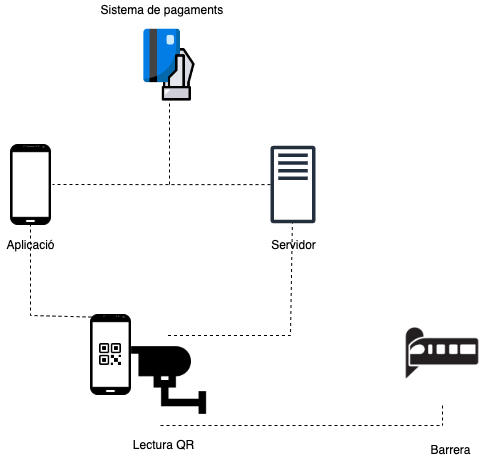
\includegraphics[scale=0.60]{Fotos/arquitectura_sistema.png}
    \end{center}
    \caption{Arquitectura del sistema}
    \label{fig:compiler_phases}
\end{figure}

\newpage
\section{Back-end}

L'arquitectura que utilitza la \emph{framework} de Laravel es basa en el MVC (Model-Vista-Controlador),
feta servir per la implementació d'interfícies d'usuari, dades i la lògica.
Aquesta separació ens dóna una millor divisió de treball i millora el manteniment.
\begin{itemize}
    \item Model: és qui defineix quines dades ha de tenir l'aplicació i les modifica. Si aquestes canvien, notifiquen a la vista.
    \item Vista: com s'han de mostrar les dades a l'aplicació per a l'usuari, és el disseny i la presentació.
    \item Controlador: on conté la lògica que actualitza el model. És la resposta a la so\l.licitud que fa l'usuari.
    Es comunica amb el model.
\end{itemize}

\begin{figure}[H]
    \begin{center}
        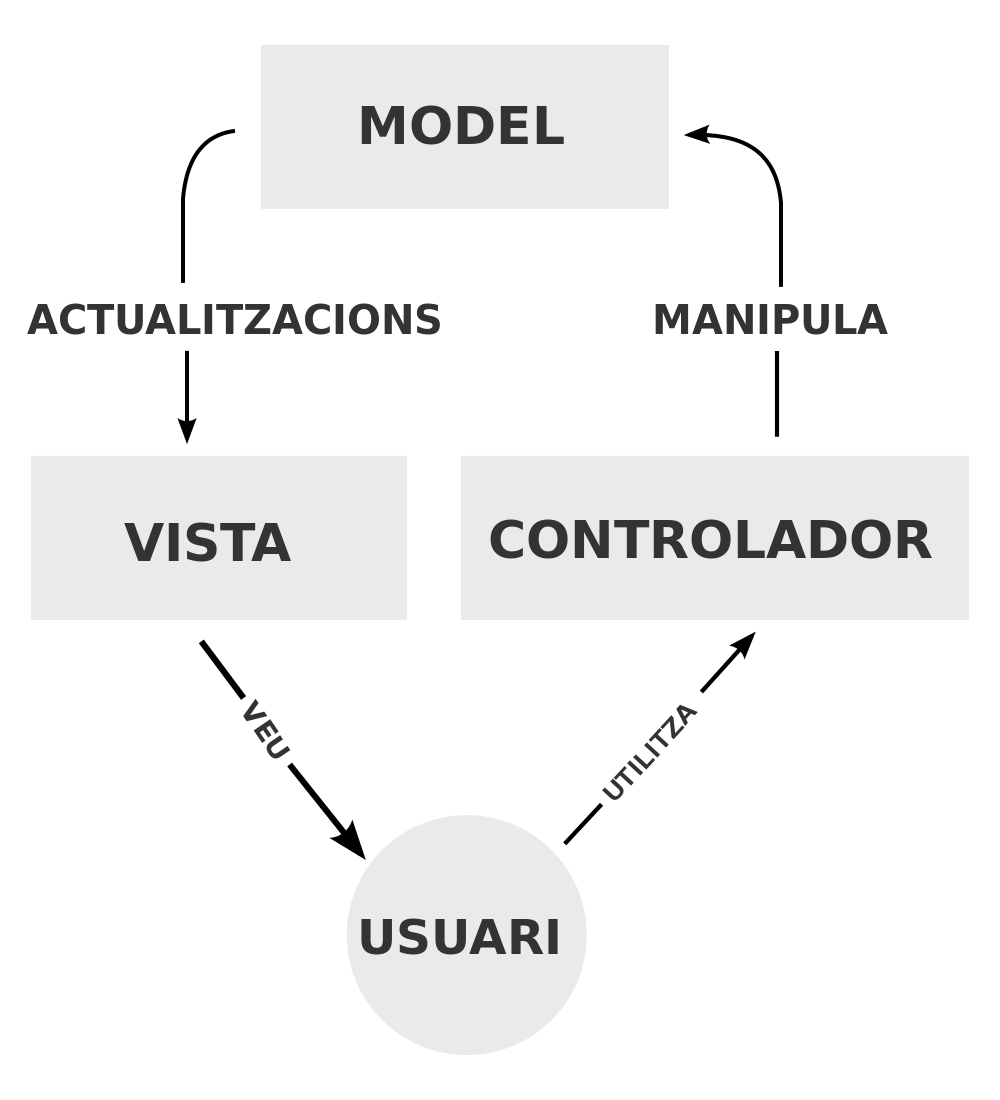
\includegraphics[scale=0.20]{Fotos/arquitectura_mvc.png}
    \end{center}
    \caption{Relació entre els elements del model MVC \autocite{mvc}}
    \label{fig:compiler_phases}
\end{figure}

\section{Front-end}

El \emph{front-end} conjuntament amb la llibreria de React la qual crea components independents
que cada un d'ells és una peça on l'usuari pot interactuar. S'encarrega de crear un espai personal
per l'usuari. Generar els diferents codis QR per l'accés o la sortida del pàrquing.
Mostrar la informació sobre l'aparcament. Fer pagaments d'una forma senzilla i amb seguretat.
A més a més disposa d'un apartat per l'administració on hi ha una part de configuració i un recull de dades.

\section{Barrera}

La Raspberry Pi a través de la càmera s'encarrega de detectar diferents codis QR. Aquests, són els
que s'han generat amb l'aplicació del \emph{front-end}. Aquesta detecció implica que la barrera
actuï de diferent manera, pujant-la o baixant-la en funció del tipus del codi QR generat.
Per aconseguir aquest efecte s'ha emprat una màquina d'estats \autocite{maq_estats}.